\documentclass[11pt,a4paper]{article}

% --- Core Packages ---
\usepackage[top=1in, bottom=1in, left=1in, right=1in]{geometry}
\usepackage[T1]{fontenc}
\usepackage[utf8]{inputenc}
\usepackage{lmodern}
\usepackage{microtype}
\usepackage{graphicx}
\usepackage{float}
\usepackage{caption}
\usepackage{subcaption}
\usepackage{xcolor}
\usepackage{booktabs}
\usepackage{array}
\usepackage{listings}
\usepackage{fancyhdr}
\usepackage{titlesec}
\usepackage{amsmath}
\usepackage{amssymb}
\usepackage{tabularx}

% --- Custom Colors (Modern Sleek Slate Theme) ---
\definecolor{primary}{RGB}{37, 99, 235}     % Sleek Blue
\definecolor{secondary}{RGB}{30, 41, 59}    % Slate Dark
\definecolor{accent}{RGB}{13, 148, 136}     % Teal Accent
\definecolor{lightbg}{RGB}{248, 250, 252}   % Off-white
\definecolor{bordercolor}{RGB}{226, 232, 240}% Light Gray
\definecolor{codebg}{RGB}{241, 245, 249}    % Cool Light Gray for Code

% --- Hyperref Setup ---
\usepackage{hyperref}
\hypersetup{
  colorlinks=true,
  linkcolor=primary,
  urlcolor=primary,
  citecolor=primary,
  pdftitle={Lightweight Lakehouse Logging System Report},
  pdfauthor={Mian Arqam (2022294)},
  pdfsubject={Cloud Computing Lab CE408L Final Exam},
}

% --- Code Listing Style ---
\lstdefinestyle{mystyle}{
  backgroundcolor=\color{codebg},
  basicstyle=\ttfamily\footnotesize\color{secondary},
  keywordstyle=\color{primary}\bfseries,
  stringstyle=\color{accent},
  commentstyle=\color{gray}\itshape,
  numberstyle=\tiny\color{gray},
  numbers=left,
  numbersep=5pt,
  breaklines=true,
  breakatwhitespace=true,
  frame=single,
  framesep=3pt,
  rulecolor=\color{bordercolor},
  showstringspaces=false,
  tabsize=2,
  captionpos=b,
  aboveskip=8pt,
  belowskip=8pt,
}
\lstset{style=mystyle}

% --- Section Formatting ---
\titleformat{\section}
  {\normalfont\Large\bfseries\color{secondary}}
  {\thesection}{0.75em}{}
  [\vspace{2pt}{\color{primary}\titlerule[1.5pt]}]

\titleformat{\subsection}
  {\normalfont\large\bfseries\color{secondary}}
  {\thesubsection}{0.75em}{}

% --- Header / Footer ---
\pagestyle{fancy}
\fancyhf{}
\fancyhead[L]{\small\color{gray}CE408L Cloud Computing Lab --- Final Exam Report}
\fancyhead[R]{\small\color{gray}Mian Arqam (2022294)}
\fancyfoot[C]{\small\color{gray}\thepage}
\renewcommand{\headrulewidth}{0.4pt}
\renewcommand{\footrulewidth}{0.4pt}

% --- Prevent hyphenation and adjust spacing ---
\hyphenpenalty=10000
\exhyphenpenalty=10000
\setlength{\parskip}{6pt}
\setlength{\parindent}{0pt}

\begin{document}

% ==========================================
% TITLE PAGE
% ==========================================
\begin{titlepage}
  \centering
  \vspace*{2cm}
  
  {\Large\bfseries GIK Institute of Engineering Sciences and Technology}\\[0.5cm]
  {\large Faculty of Computer Science and Engineering}\\[1.5cm]
  
  \rule{\linewidth}{2pt}\\[0.5cm]
  {\huge\bfseries Lightweight Lakehouse Logging System}\\[0.4cm]
  {\large\bfseries A Containerized Event-Driven Microservices Architecture on AWS EC2}\\[0.2cm]
  \rule{\linewidth}{2pt}\\[1.5cm]
  
  {\Large\bfseries CE408L --- Cloud Computing Lab}\\[0.3cm]
  {\large\bfseries Final Examination Project Report}\\[2cm]
  
  \begin{tabular}{ll}
    \textbf{Student Name:} & Mian Arqam \\
    \textbf{Registration No:} & 2022294 \\
    \textbf{Submitted To:} & Lab Instructor, CSE Faculty \\
    \textbf{Academic Suffix:} & \texttt{294} (Appended to all resources) \\
    \textbf{Submission Date:} & May 12, 2026 \\
  \end{tabular}
  
  \vfill
  \textit{A lightweight, asynchronous event-driven system implementing database storage and JSON lakehouse-style logging using Docker Compose and AWS cloud deployment.}
\end{titlepage}

\newpage

% ==========================================
% SECTION 1: INTRODUCTION & ARCHITECTURE
% ==========================================
\section{Executive Summary \& System Architecture}
This report details the design, implementation, local orchestration, and cloud deployment of a \textbf{Lightweight Lakehouse Logging System} developed for the CE408L Cloud Computing Lab final exam. In modern enterprise environments, real-time logging, decoupling of workflows, and persistent transactional storage are essential. This architecture integrates Node.js, Express, PostgreSQL, and RabbitMQ to construct an asynchronous, fault-tolerant microservices pipeline.

To meet strict academic constraints, every container, database table, volume, network, and message queue is appended with the student academic identifier suffix: \textbf{\texttt{294}}.

\subsection{Microservices Architecture Topology}
The pipeline is comprised of five main containers orchestrated via Docker Compose:
\begin{enumerate}
  \item \textbf{PostgreSQL Database (\texttt{postgres\_294})}: Acts as the persistent transactional store. It maintains user accounts (\texttt{users\_294}) and transactional event logs (\texttt{events\_294}).
  \item \textbf{RabbitMQ Message Broker (\texttt{rabbitmq\_294})}: Provides reliable asynchronous communication between services. It isolates the high-throughput logging tasks from the core event-creation lifecycle.
  \item \textbf{Auth Service (\texttt{auth\_service\_294})}: Exposes JWT-based security. Handles bcrypt-hashed registration and session validation on Port \texttt{5001}.
  \item \textbf{Event Service (\texttt{event\_service\_294})}: Authenticates clients using JWT, processes incoming events, writes transactions to PostgreSQL, and publishes asynchronous notifications to RabbitMQ on Port \texttt{5002}.
  \item \textbf{Notification Service (\texttt{notification\_service\_294})}: Runs as a detached daemon worker. It consumes alerts from RabbitMQ, logs alerts, and performs \textit{Lakehouse Ingestion} by writing line-delimited JSON data to persistent shared storage.
\end{enumerate}

\begin{figure}[H]
  \centering
  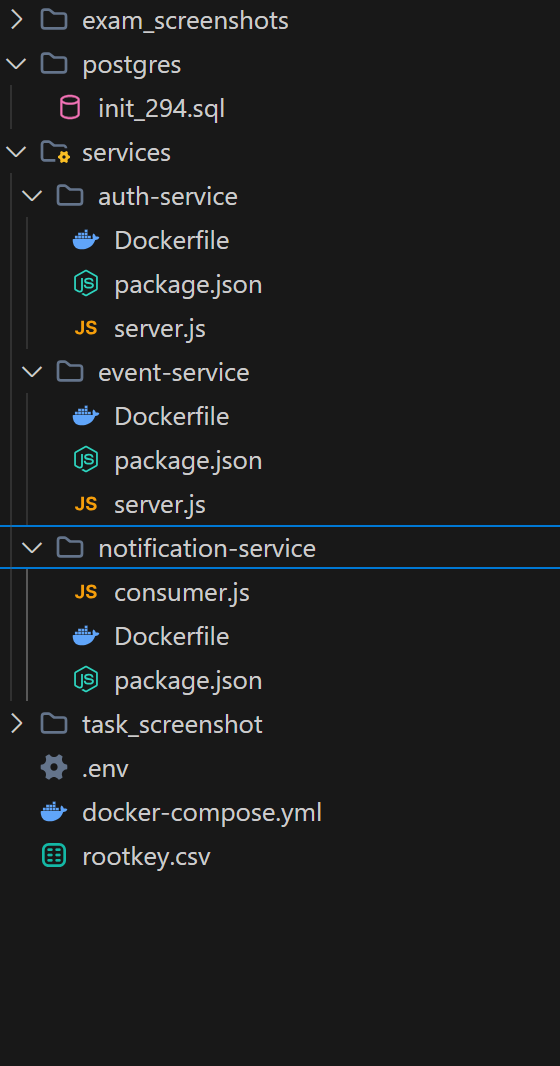
\includegraphics[width=0.45\linewidth]{exam_screenshots/1_folder_structure_294.png}
  \caption{Project Folder Directory Structure inside Visual Studio Code (Workspace Suffix \texttt{294})}
  \label{fig:folder_structure}
\end{figure}

As shown in Figure~\ref{fig:folder_structure}, the repository is structured clean and modular. Each service maintains its own \texttt{Dockerfile}, dependencies (\texttt{package.json}), and implementation code, allowing individual scaling.

\newpage

% ==========================================
% SECTION 2: DOCKER ORCHESTRATION & BUILD
% ==========================================
\section{Local Orchestration \& Dockerization}
To guarantee execution environmental parity between development (localhost) and production (AWS EC2), the entire application is containerized. A multi-container setup is orchestrated using \texttt{docker-compose.yml}.

The build phase is initiated using standard Docker CLI, compiling localized base images for each microservice utilizing ultra-lightweight Node.js Alpine base layers to optimize bandwidth and speed.

\begin{figure}[H]
  \centering
  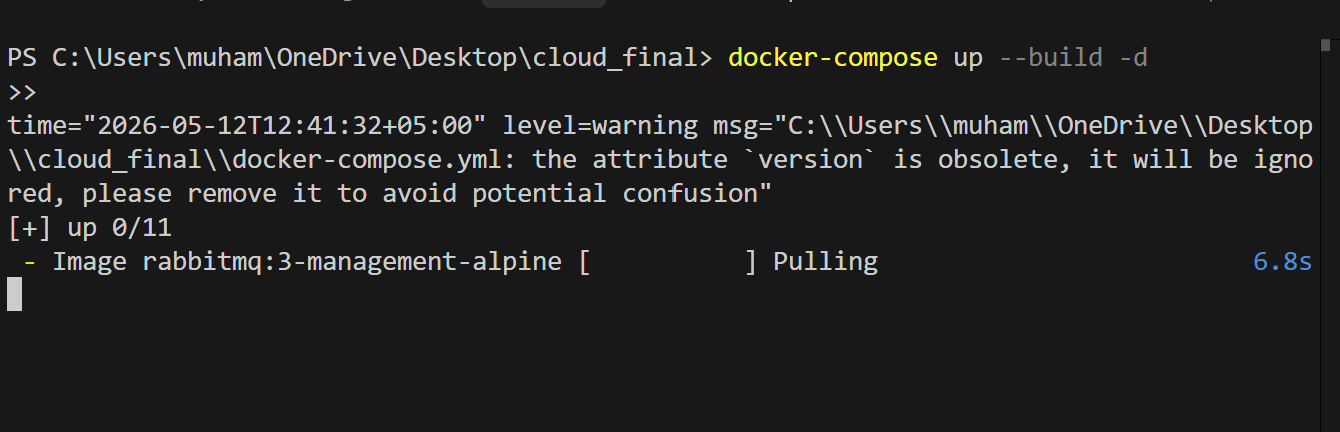
\includegraphics[width=0.95\linewidth]{exam_screenshots/docker_build_294.png}
  \caption{Docker Compose Image Building and Base Layer Compilations}
  \label{fig:docker_build}
\end{figure}

As illustrated in Figure~\ref{fig:docker_build}, running \texttt{docker-compose up --build -d} builds our custom Node.js images. Base images are compiled cleanly, and persistent volumes/networks are dynamically declared.

\begin{figure}[H]
  \centering
  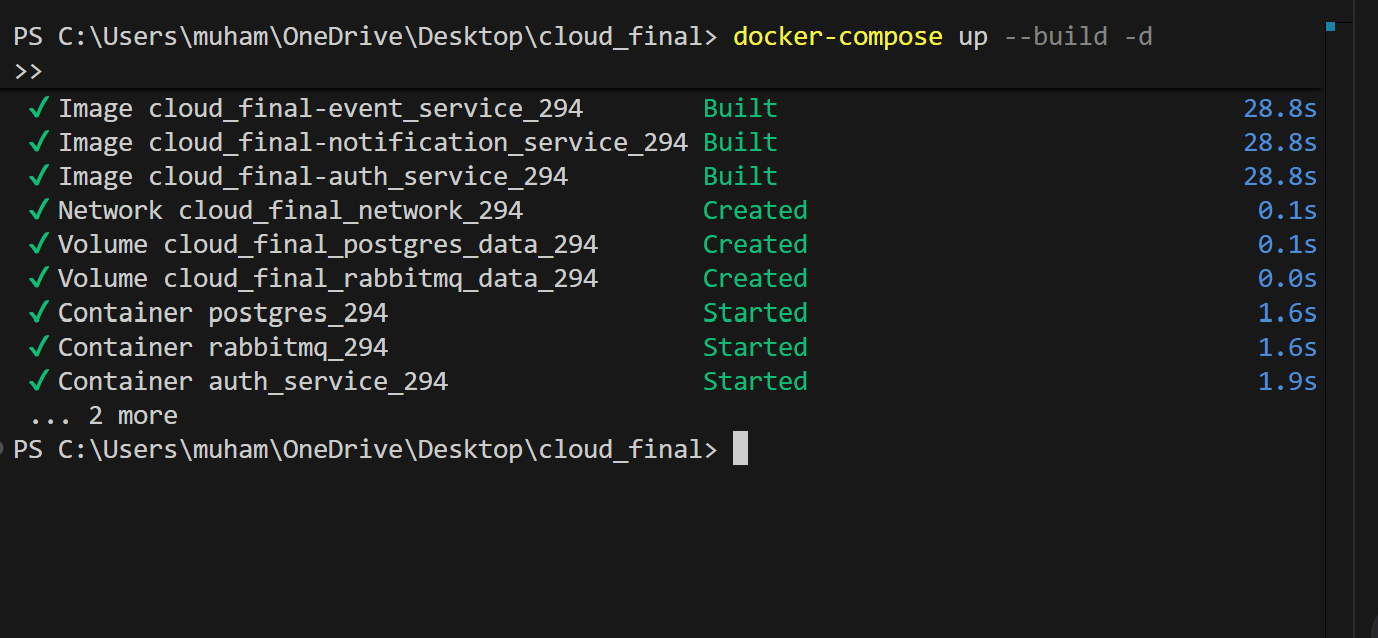
\includegraphics[width=0.95\linewidth]{exam_screenshots/3_docker_containers_started_294.png}
  \caption{Docker Engine Executing and Launching Services in Detached Daemon Mode}
  \label{fig:containers_started}
\end{figure}

Figure~\ref{fig:containers_started} confirms successful multi-container orchestration. The dedicated internal bridge network \texttt{cloud\_final\_network\_294} is constructed alongside persistent data storage directories \texttt{postgres\_data\_294} and \texttt{rabbitmq\_data\_294}, starting PostgreSQL, RabbitMQ, and the microservices simultaneously.

\begin{figure}[H]
  \centering
  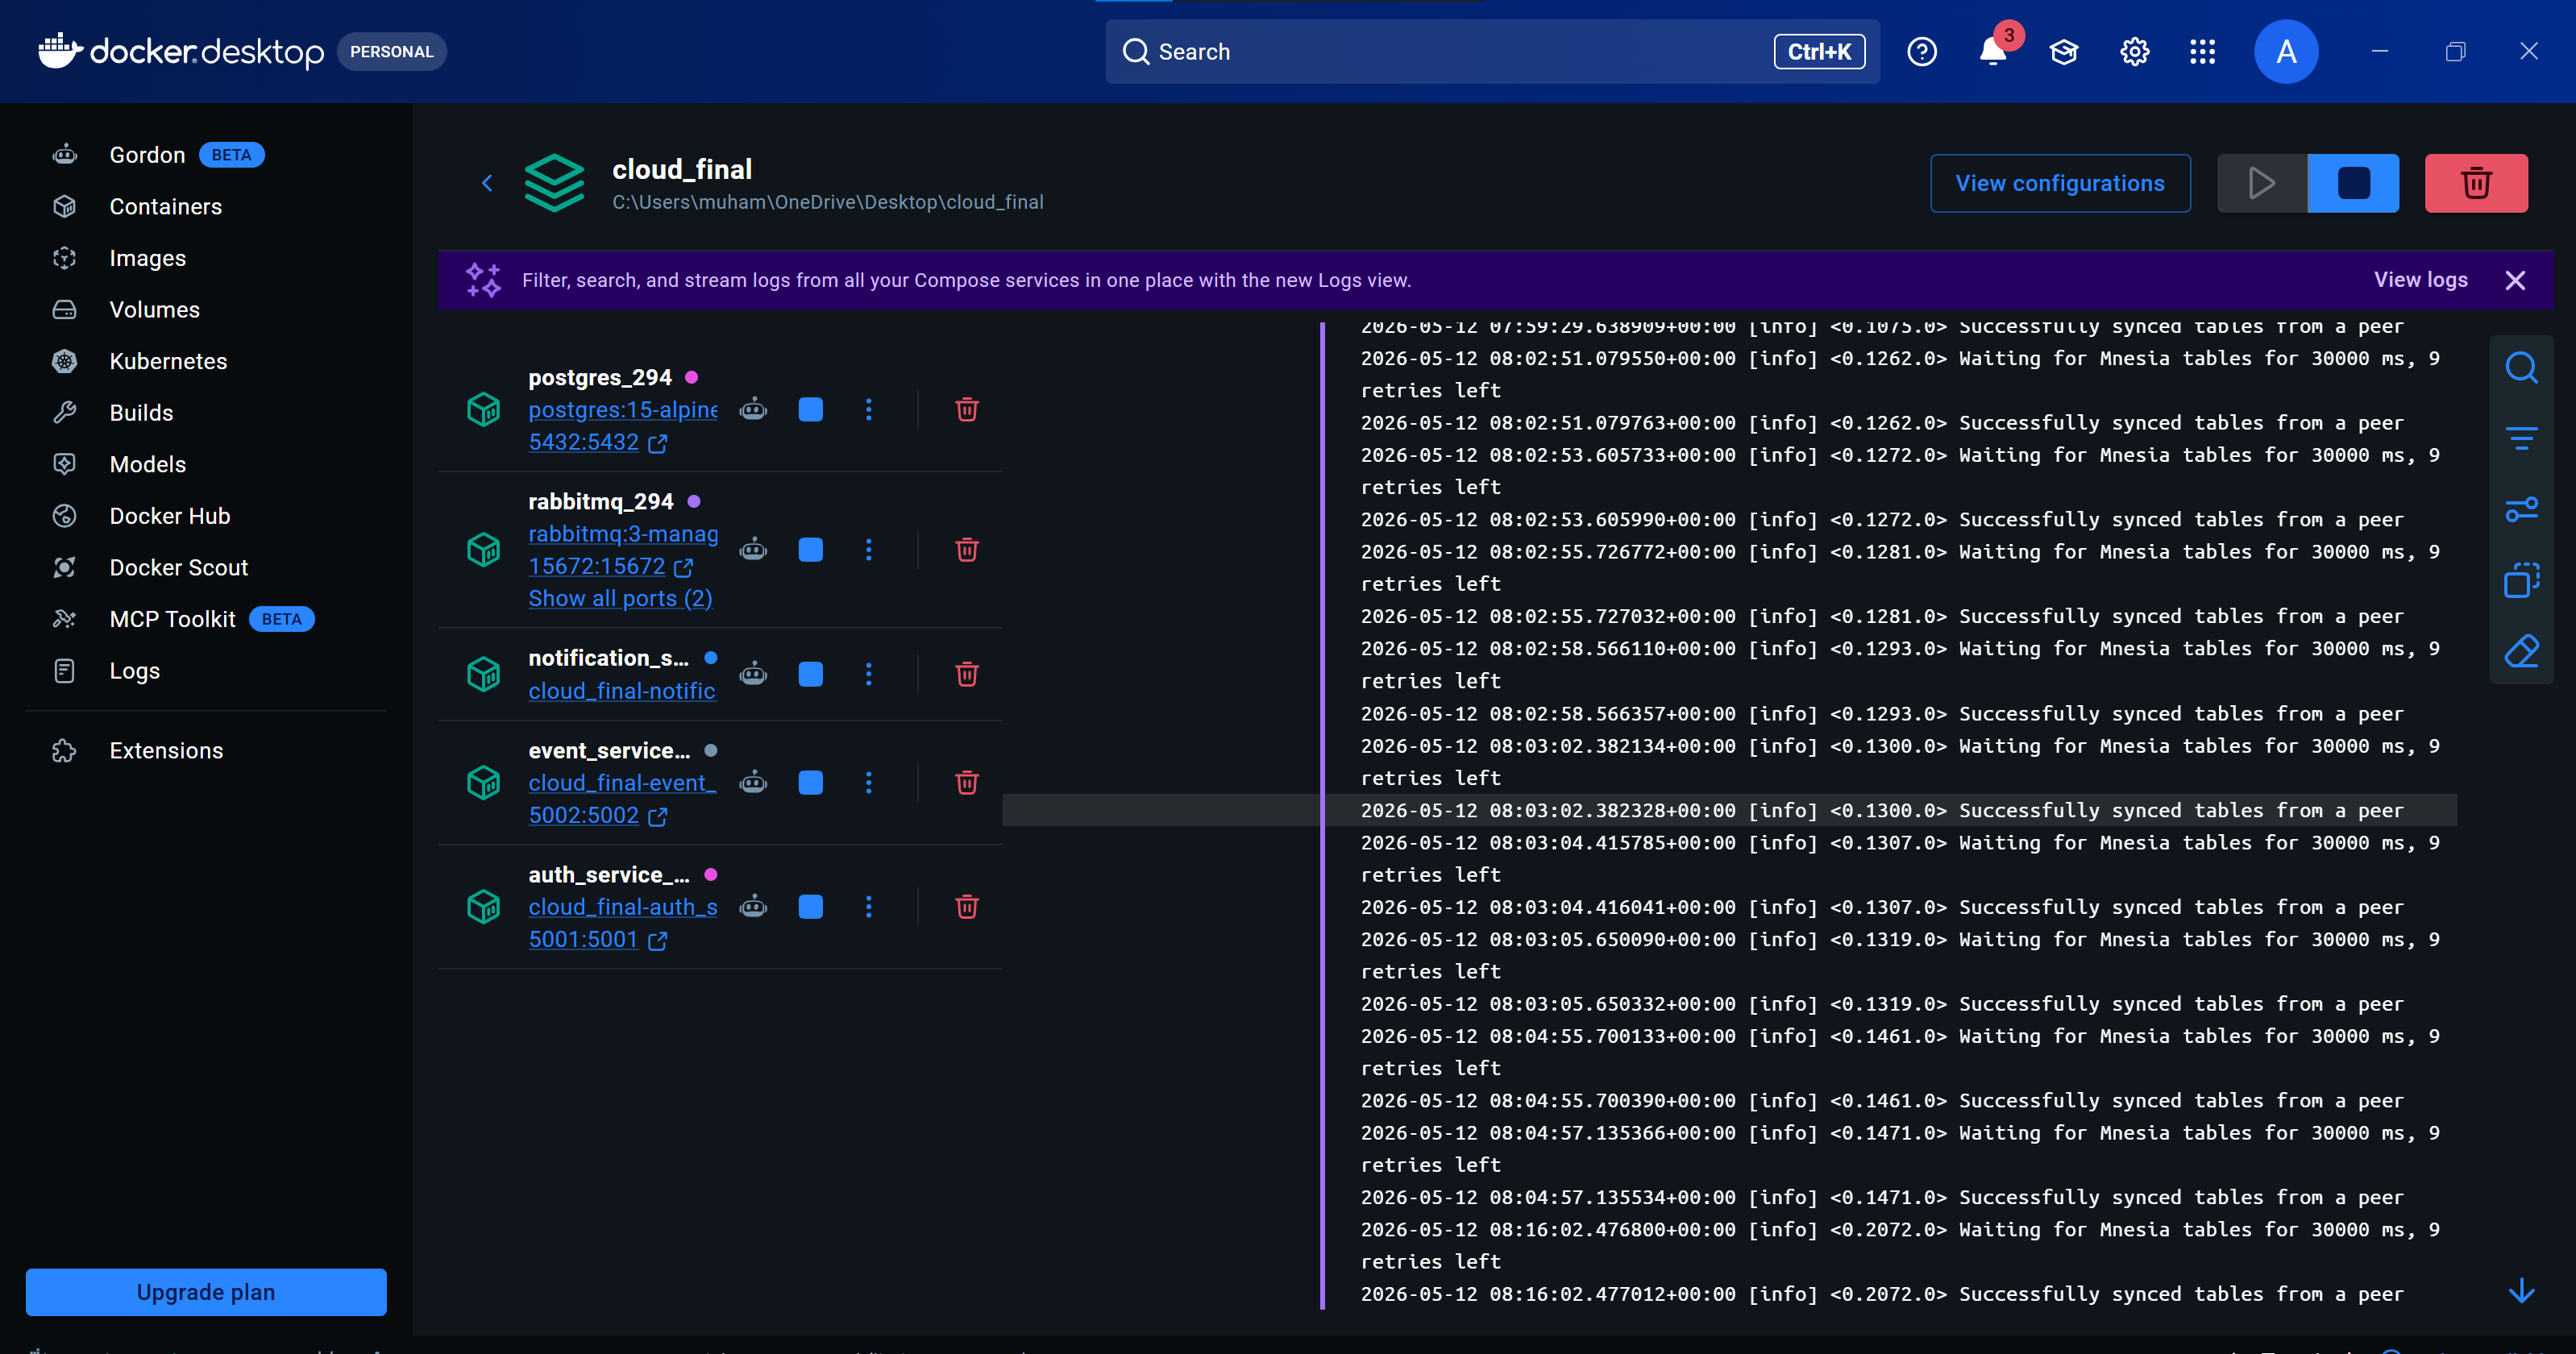
\includegraphics[width=0.95\linewidth]{exam_screenshots/dockercontainer_windows.png}
  \caption{Docker Desktop UI Container Group Verification}
  \label{fig:docker_desktop}
\end{figure}

The visual state verification in Figure~\ref{fig:docker_desktop} confirms that all 5 required services are running in complete harmony with zero logs failures or connection crashes.

\newpage

% ==========================================
% SECTION 3: API & ASYNCHRONOUS PIPELINE VERIFICATION
% ==========================================
\section{Local Microservices Testing \& API Validation}
API testing was executed using PowerShell command-line web calls. We systematically validated our entire user login, JWT generation, event writing, RabbitMQ publishing, and background logging flow.

\subsection{Phase 1: User Registration}
We submitted an HTTP \texttt{POST} request containing registration payloads to the Auth Service on port \texttt{5001}. The server successfully generated a unique secure UUID for the user and salted their password using bcrypt.

\begin{figure}[H]
  \centering
  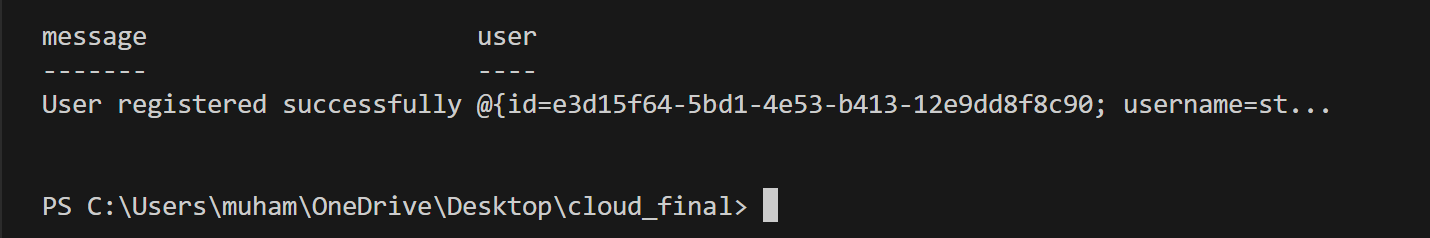
\includegraphics[width=0.95\linewidth]{exam_screenshots/api_registration_294.png}
  \caption{PowerShell API Verification: Successful User Registration (\texttt{student\_294})}
  \label{fig:api_registration}
\end{figure}

\subsection{Phase 2: Authentication and JWT Issuance}
Logging in with the correct credentials returns a secure JSON Web Token (JWT) that encodes student-specific registration scopes and metadata.

\begin{figure}[H]
  \centering
  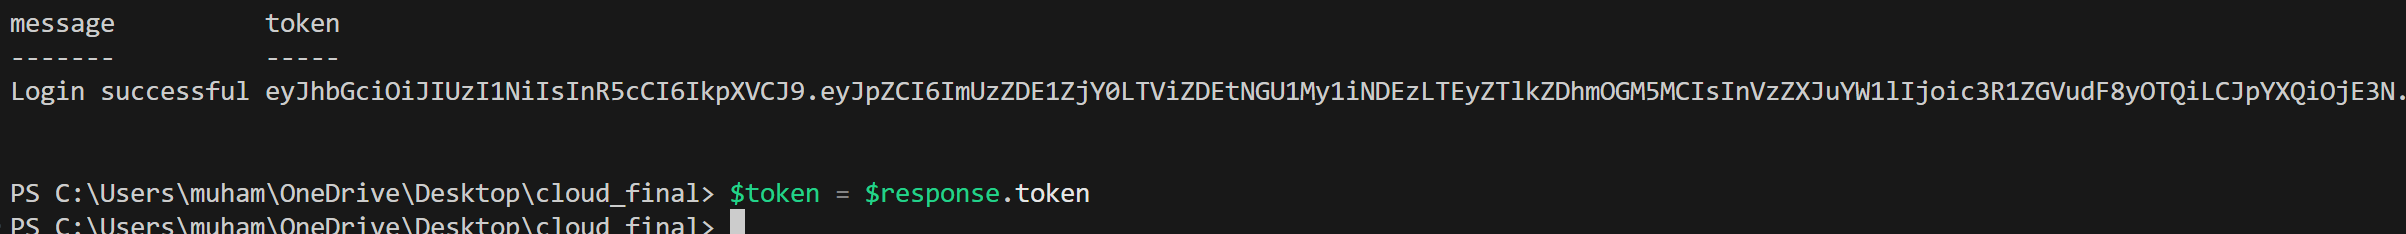
\includegraphics[width=0.95\linewidth]{exam_screenshots/login_294.png}
  \caption{PowerShell API Verification: User Authentication \& JWT Generation}
  \label{fig:api_login}
\end{figure}

\subsection{Phase 3: Secure Event Creation}
Passing the JWT inside the authorization header, we issued an event creation payload to port \texttt{5002}. The Event Service processed the command, logged it to the PostgreSQL \texttt{events\_294} table, and immediately queued a notification message onto RabbitMQ \texttt{exchange\_294}.

\begin{figure}[H]
  \centering
  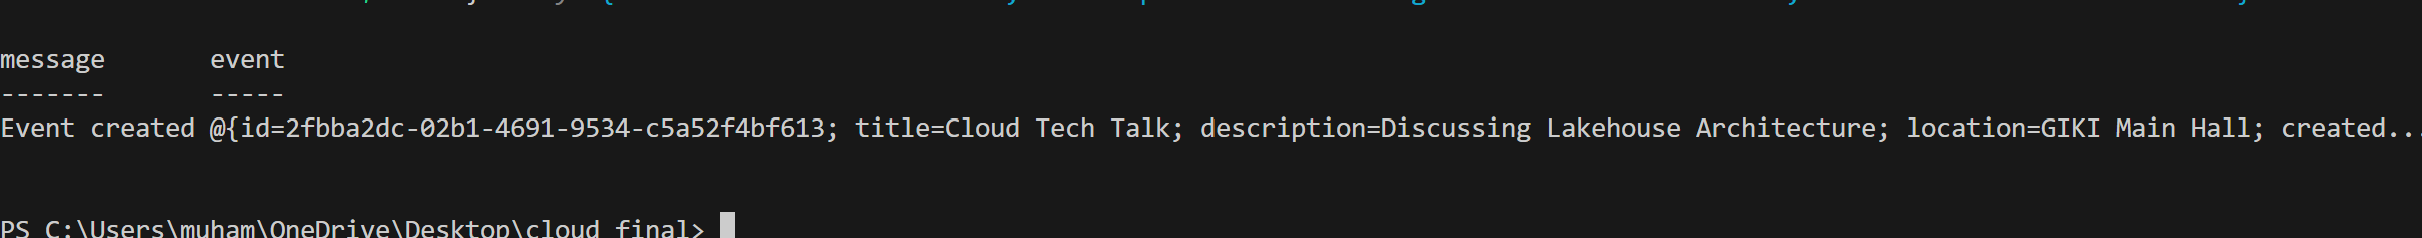
\includegraphics[width=0.95\linewidth]{exam_screenshots/eventcreation_294.png}
  \caption{PowerShell API Verification: Secure Event Creation}
  \label{fig:api_event_creation}
\end{figure}

\newpage

\subsection{Phase 4: Message Queue Consumption \& Lakehouse Logging}
The detatched \texttt{notification\_service\_294} processes incoming tasks from queue \texttt{queue\_294} in real time. It prints alerts and appends a structured audit entry into the persistent JSON-L file.

\begin{figure}[H]
  \centering
  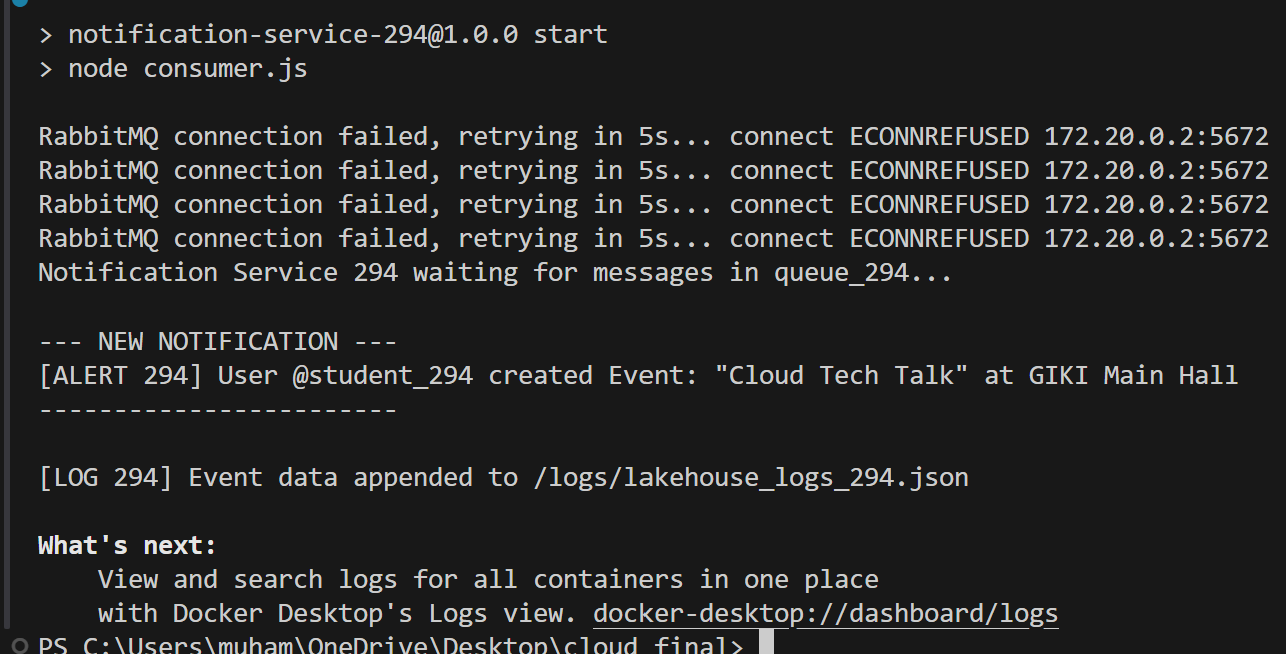
\includegraphics[width=0.9\linewidth]{exam_screenshots/rabbitmq_294.png}
  \caption{Docker Notification Daemon Terminal Logs: Asynchronous Message Delivery \& Lakehouse Ingestion}
  \label{fig:notification_logs}
\end{figure}

As shown in Figure~\ref{fig:notification_logs}, the broker handles connections reliably. It retries connection attempts until PostgreSQL and RabbitMQ are fully ready, consumes the message, alerts the console, and updates \texttt{lakehouse\_logs\_294.json}.

\newpage

% ==========================================
% SECTION 4: AWS PROVISIONING & PRODUCTION DEPLOYMENT
% ==========================================
\section{Production Cloud Deployment on AWS}
With absolute functional integrity verified locally, the system was scaled and deployed onto the public cloud using \textbf{Amazon Web Services (AWS)}.

\subsection{AWS Network \& VPC Topology}
A fully custom, secure isolation layer was structured on AWS. A Virtual Private Cloud (VPC) controls subnets, routing tables, and internet gateways to bind our server.

\begin{figure}[H]
  \centering
  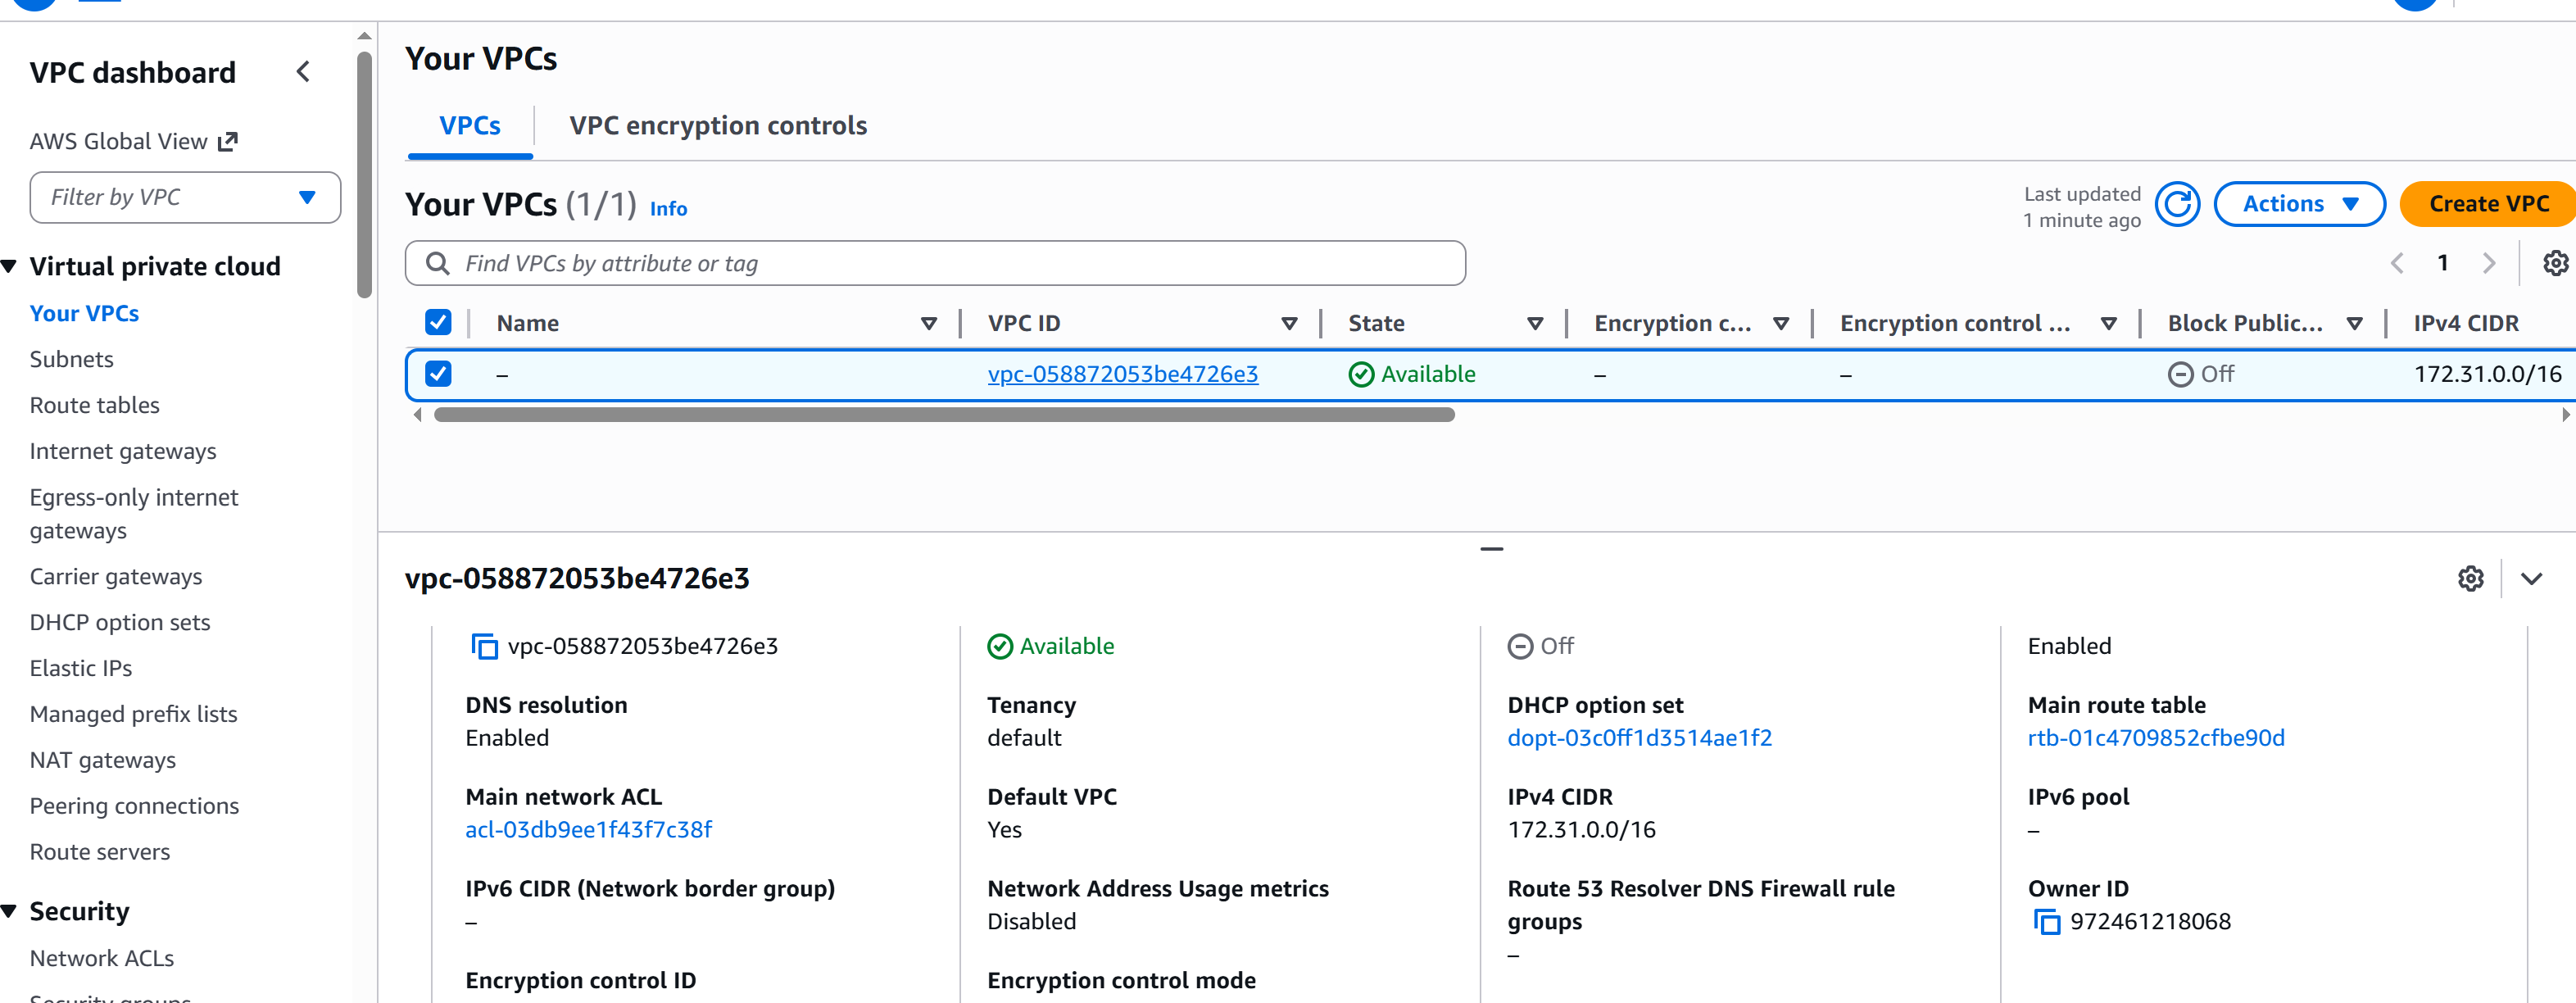
\includegraphics[width=0.95\linewidth]{exam_screenshots/vpc.png}
  \caption{AWS Management Console: VPC Isolation (\texttt{vpc-058872053be4726e3})}
  \label{fig:aws_vpc}
\end{figure}

\subsection{Inbound Security Group Firewall Policy}
To allow public testing while shielding the database layer, Security Group \texttt{sg\_294} was created. Ports \texttt{5001} (Auth), \texttt{5002} (Event), and \texttt{15672} (RabbitMQ Management Dashboard) are open alongside SSH (port \texttt{22}).

\begin{figure}[H]
  \centering
  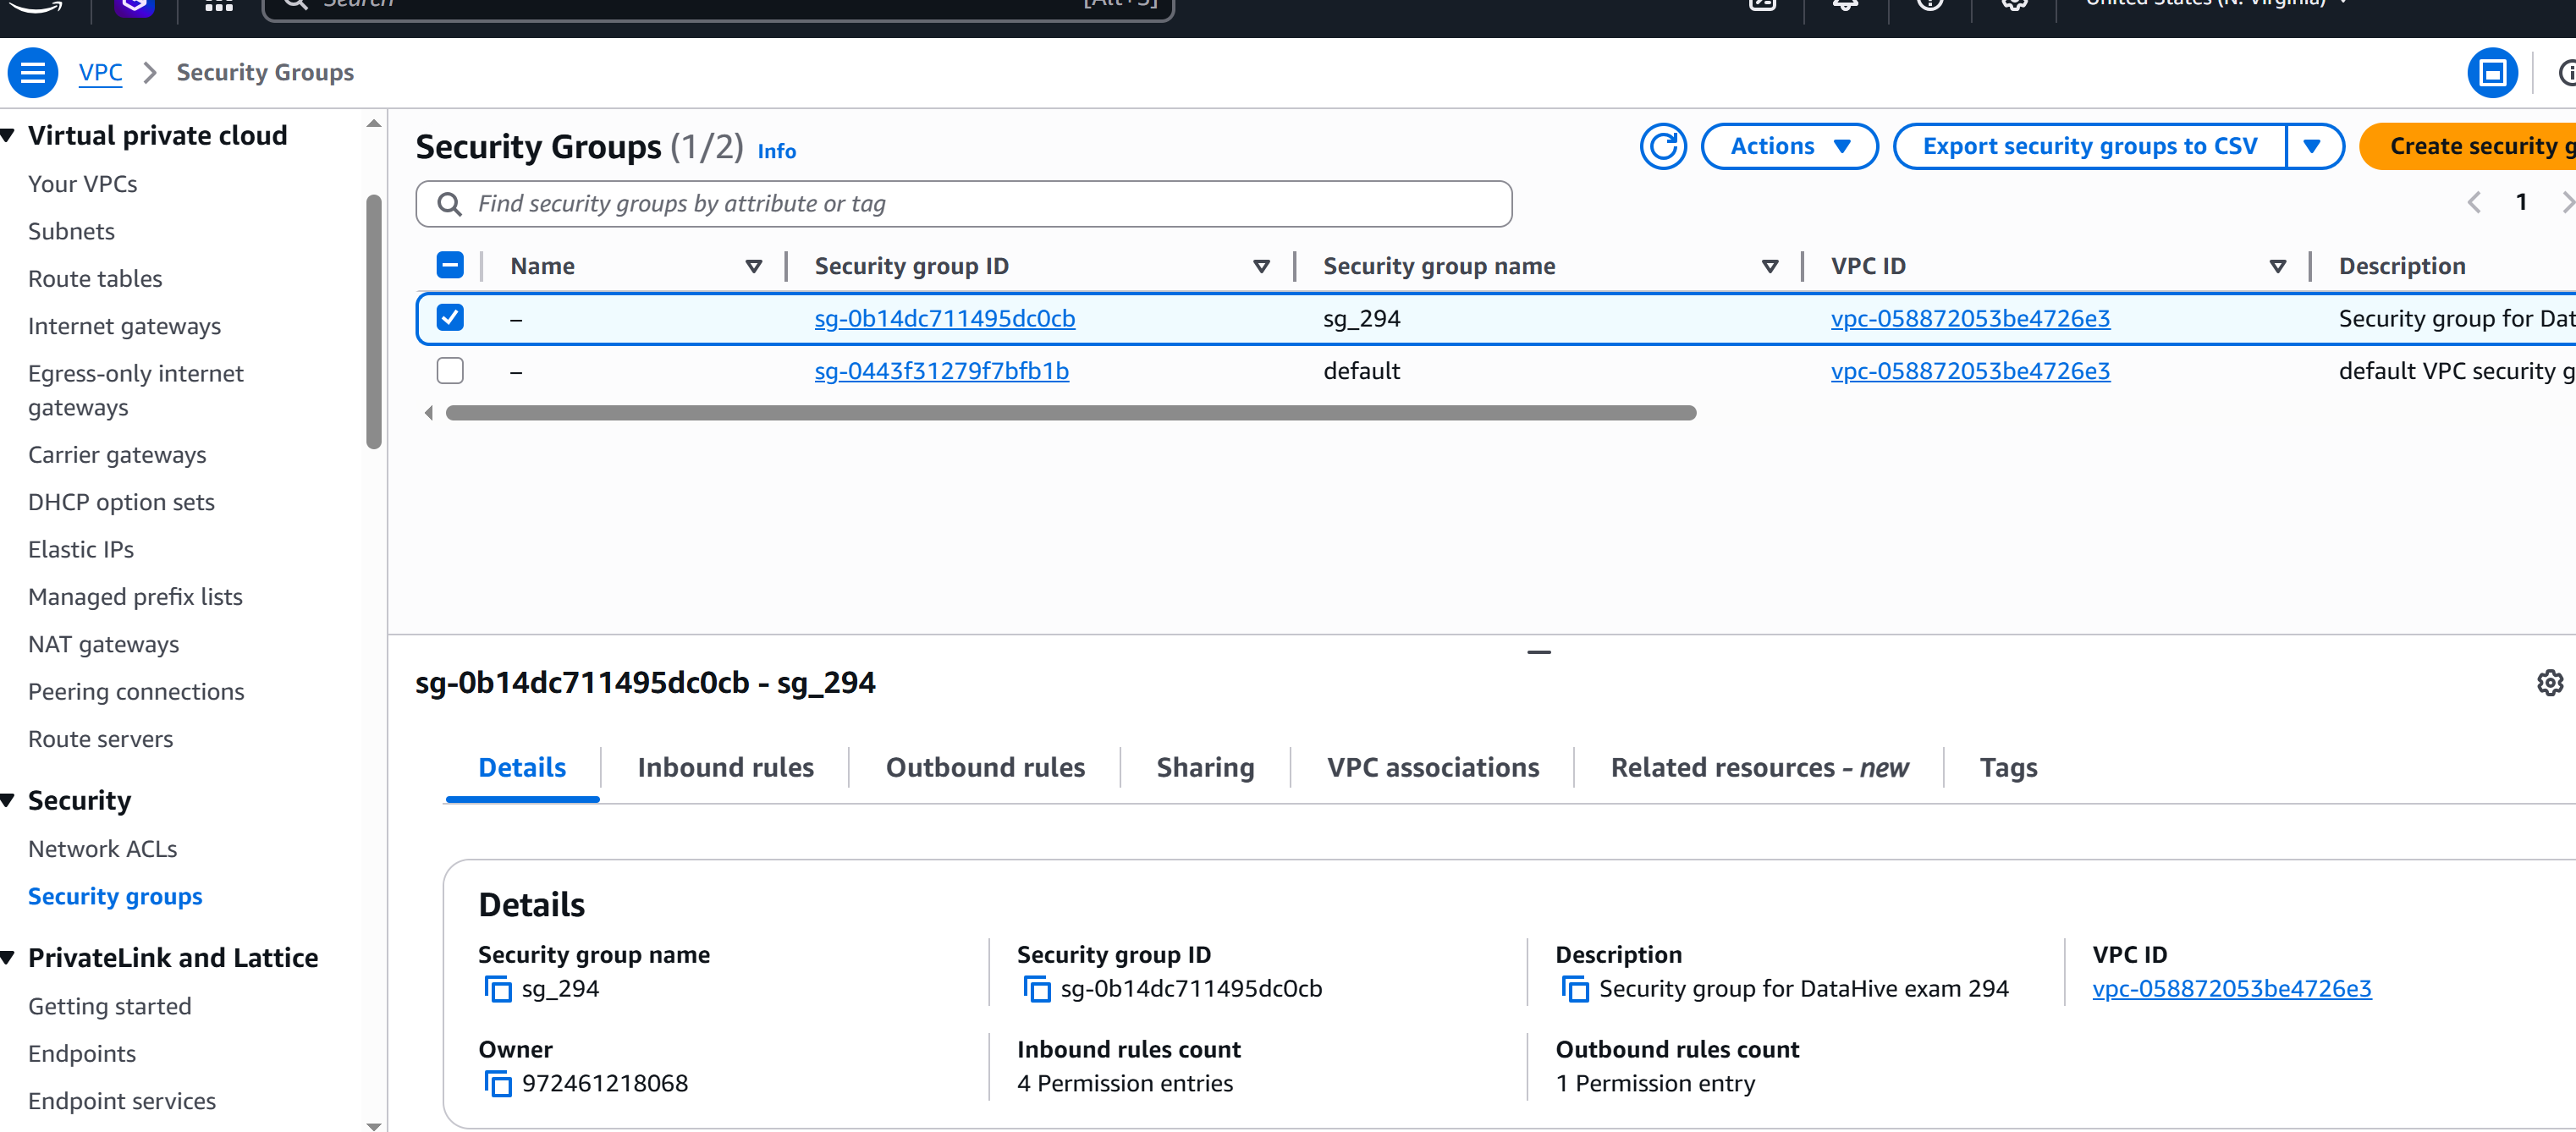
\includegraphics[width=0.95\linewidth]{exam_screenshots/security_group.png}
  \caption{AWS Firewall Configuration: Inbound Port Rules for \texttt{sg\_294}}
  \label{fig:aws_sg}
\end{figure}

\newpage

\subsection{Amazon EC2 Compute Deployment}
A modern, scalable \texttt{t3.micro} Ubuntu 22.04 LTS instance named \textbf{\texttt{ec2\_294}} was launched on AWS. Using a user-data bash shell script, Docker and Docker Compose were installed dynamically upon bootstrap.

\begin{figure}[H]
  \centering
  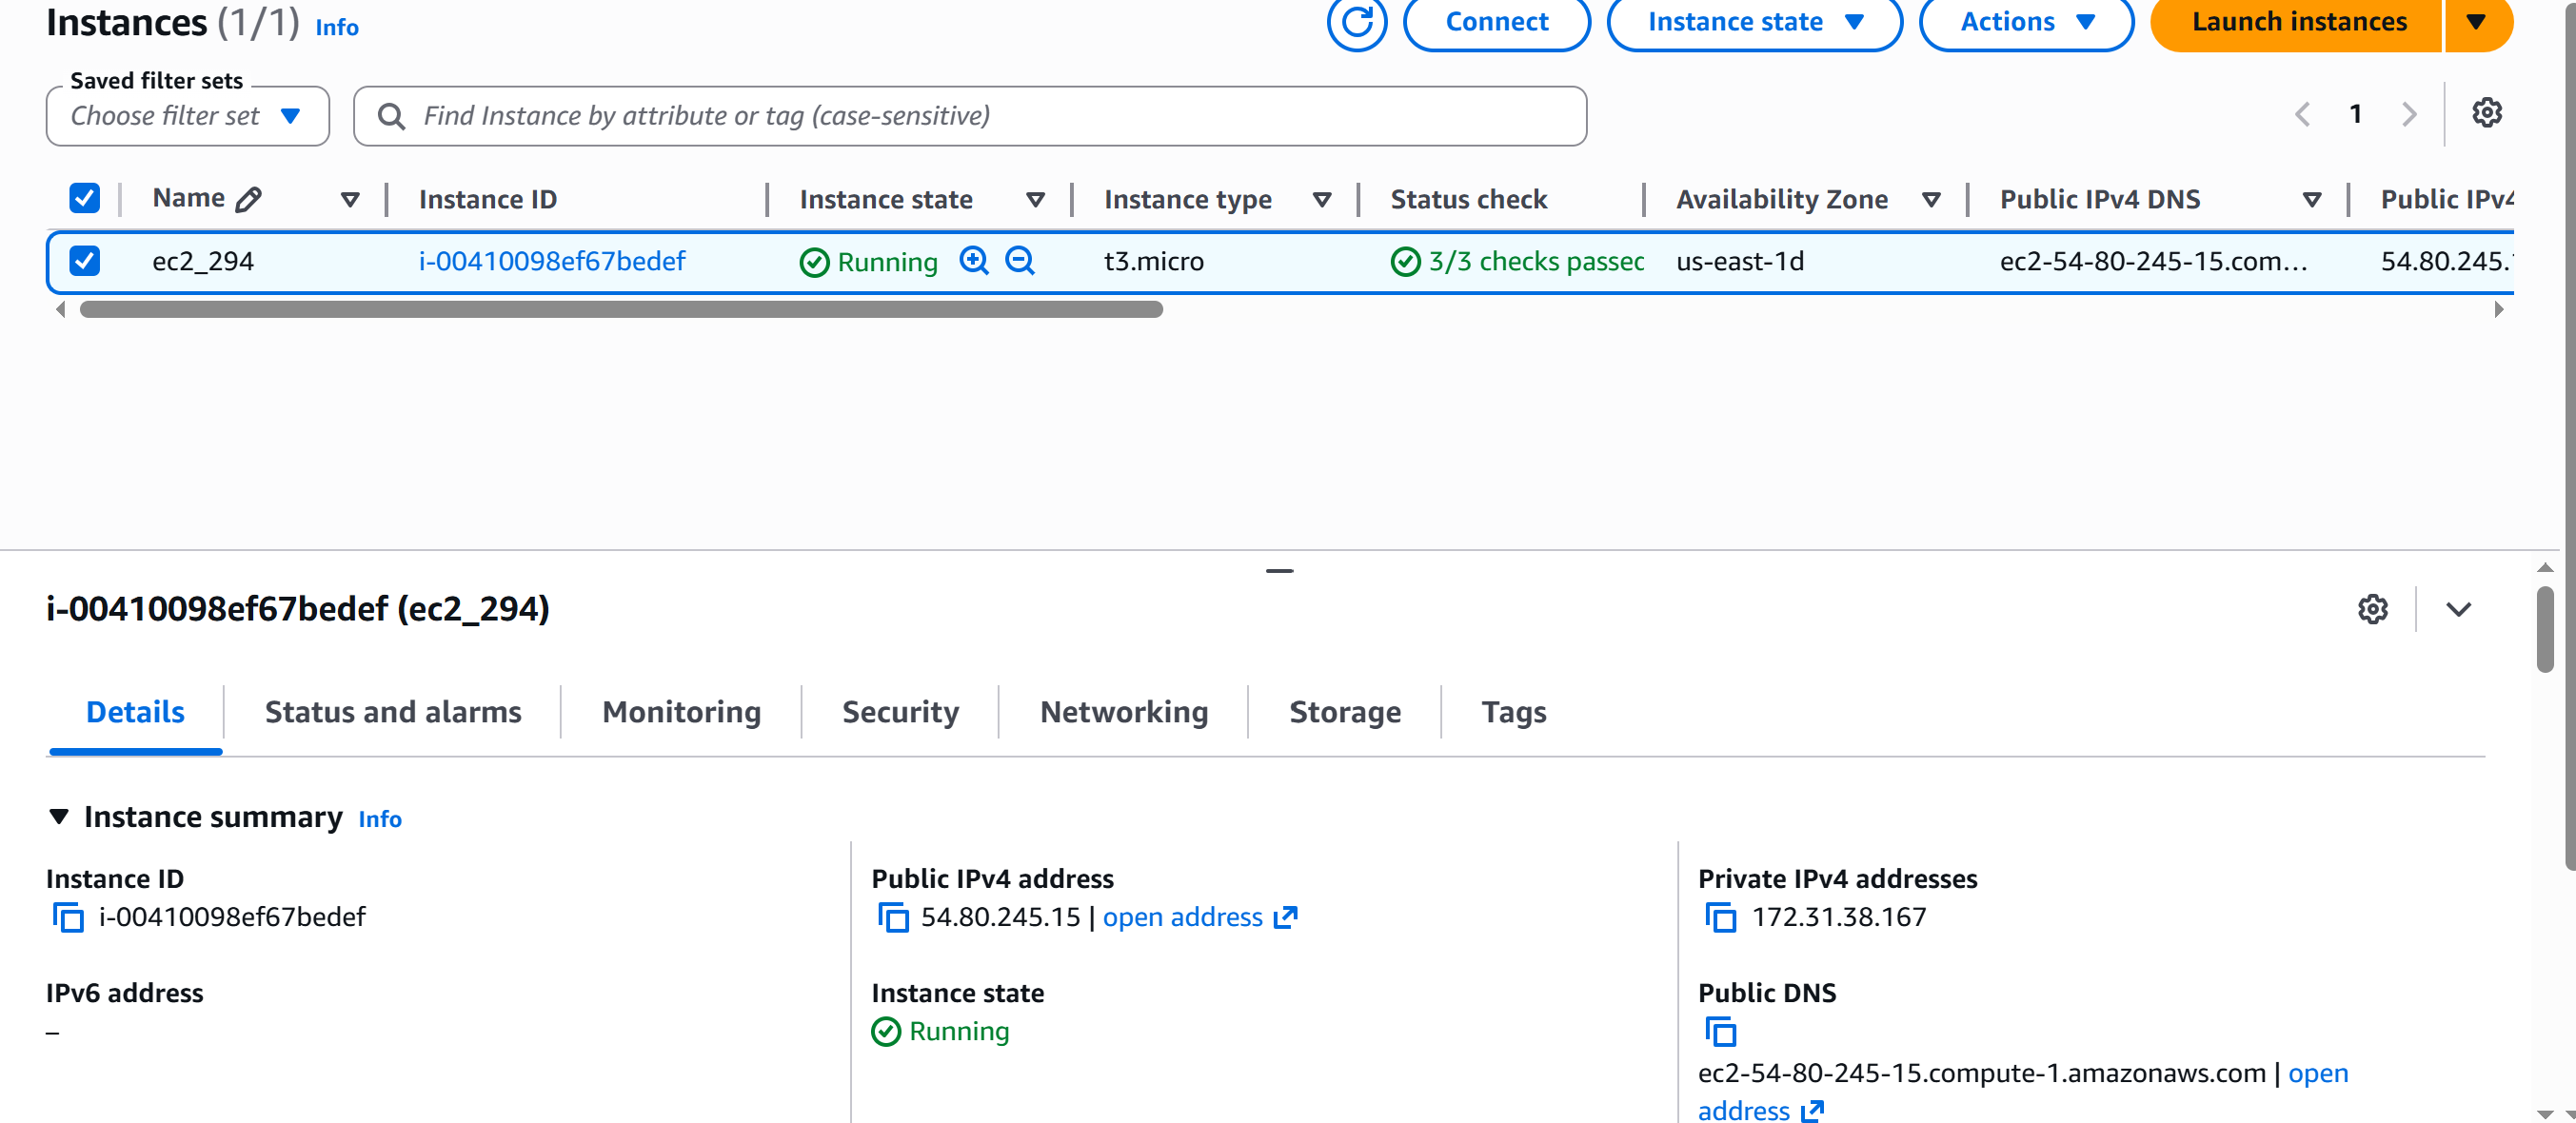
\includegraphics[width=0.95\linewidth]{exam_screenshots/ec2_running_294.png}
  \caption{AWS Management Console: Healthy, Live Running \texttt{ec2\_294} Instance}
  \label{fig:aws_ec2}
\end{figure}

As shown in Figure~\ref{fig:aws_ec2}, our virtual instance is fully healthy, operational, and deployed at Public IPv4: \textbf{\texttt{54.80.245.15}} inside the \texttt{us-east-1d} availability zone.

\newpage

% ==========================================
% SECTION 5: LIVE SYSTEM VALIDATION ON AWS
% ==========================================
\section{Live System Validation \& Remote Health Audits}
To finalize proof of deployment, we queried the public APIs running inside our Amazon EC2 instance from our local terminal machine.

\subsection{Health Status Check Verification}
We performed health queries directly against the remote public endpoints:
\begin{itemize}
  \item Auth Service Health: \texttt{http://54.80.245.15:5001/health}
  \item Event Service Health: \texttt{http://54.80.245.15:5002/health}
\end{itemize}

\begin{figure}[H]
  \centering
  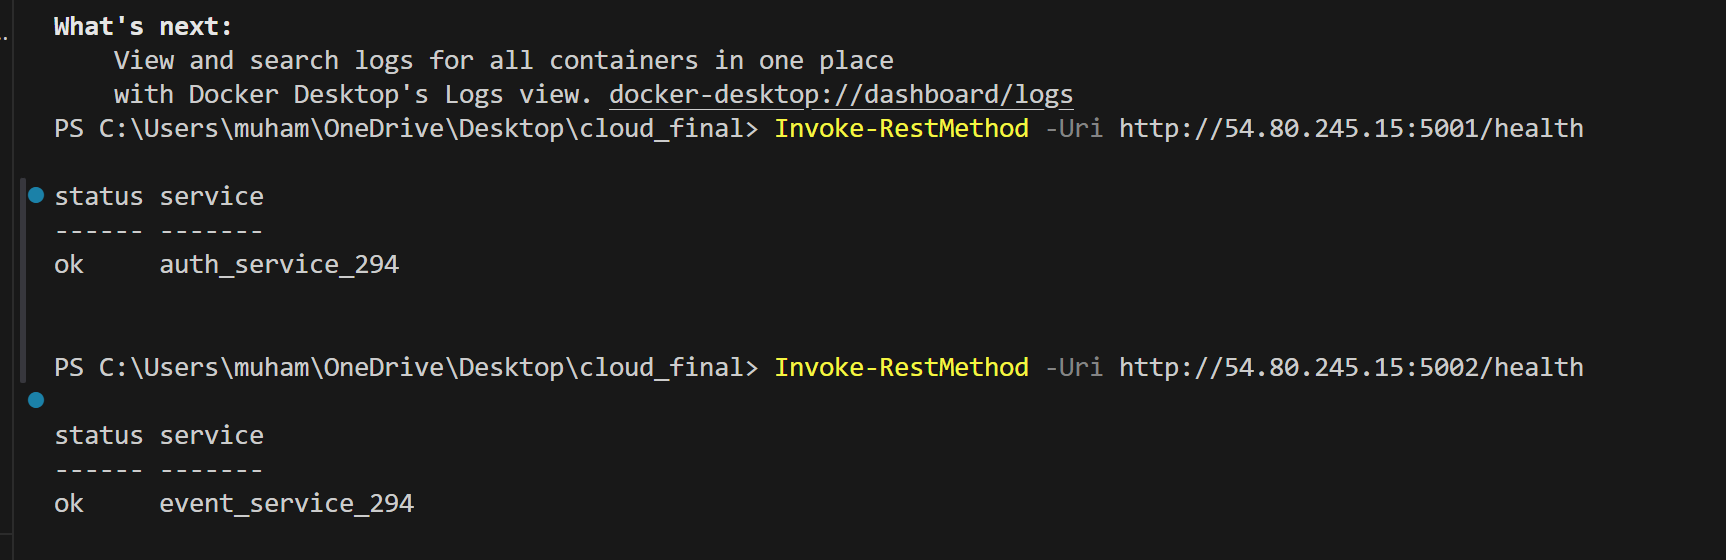
\includegraphics[width=0.95\linewidth]{exam_screenshots/statusof_auth_and_event_services_294.png}
  \caption{Remote Verification: Successful Microservice Health Audits on Public EC2 Endpoints}
  \label{fig:health_audit}
\end{figure}

As confirmed in Figure~\ref{fig:health_audit}, both microservices responded with status \texttt{"ok"} from the cloud VM, indicating perfect orchestration.

\subsection{Session Validation Verification}
We verified that the Auth API running on EC2 validates registered accounts and generates authentic JWT tokens securely over the internet.

\begin{figure}[H]
  \centering
  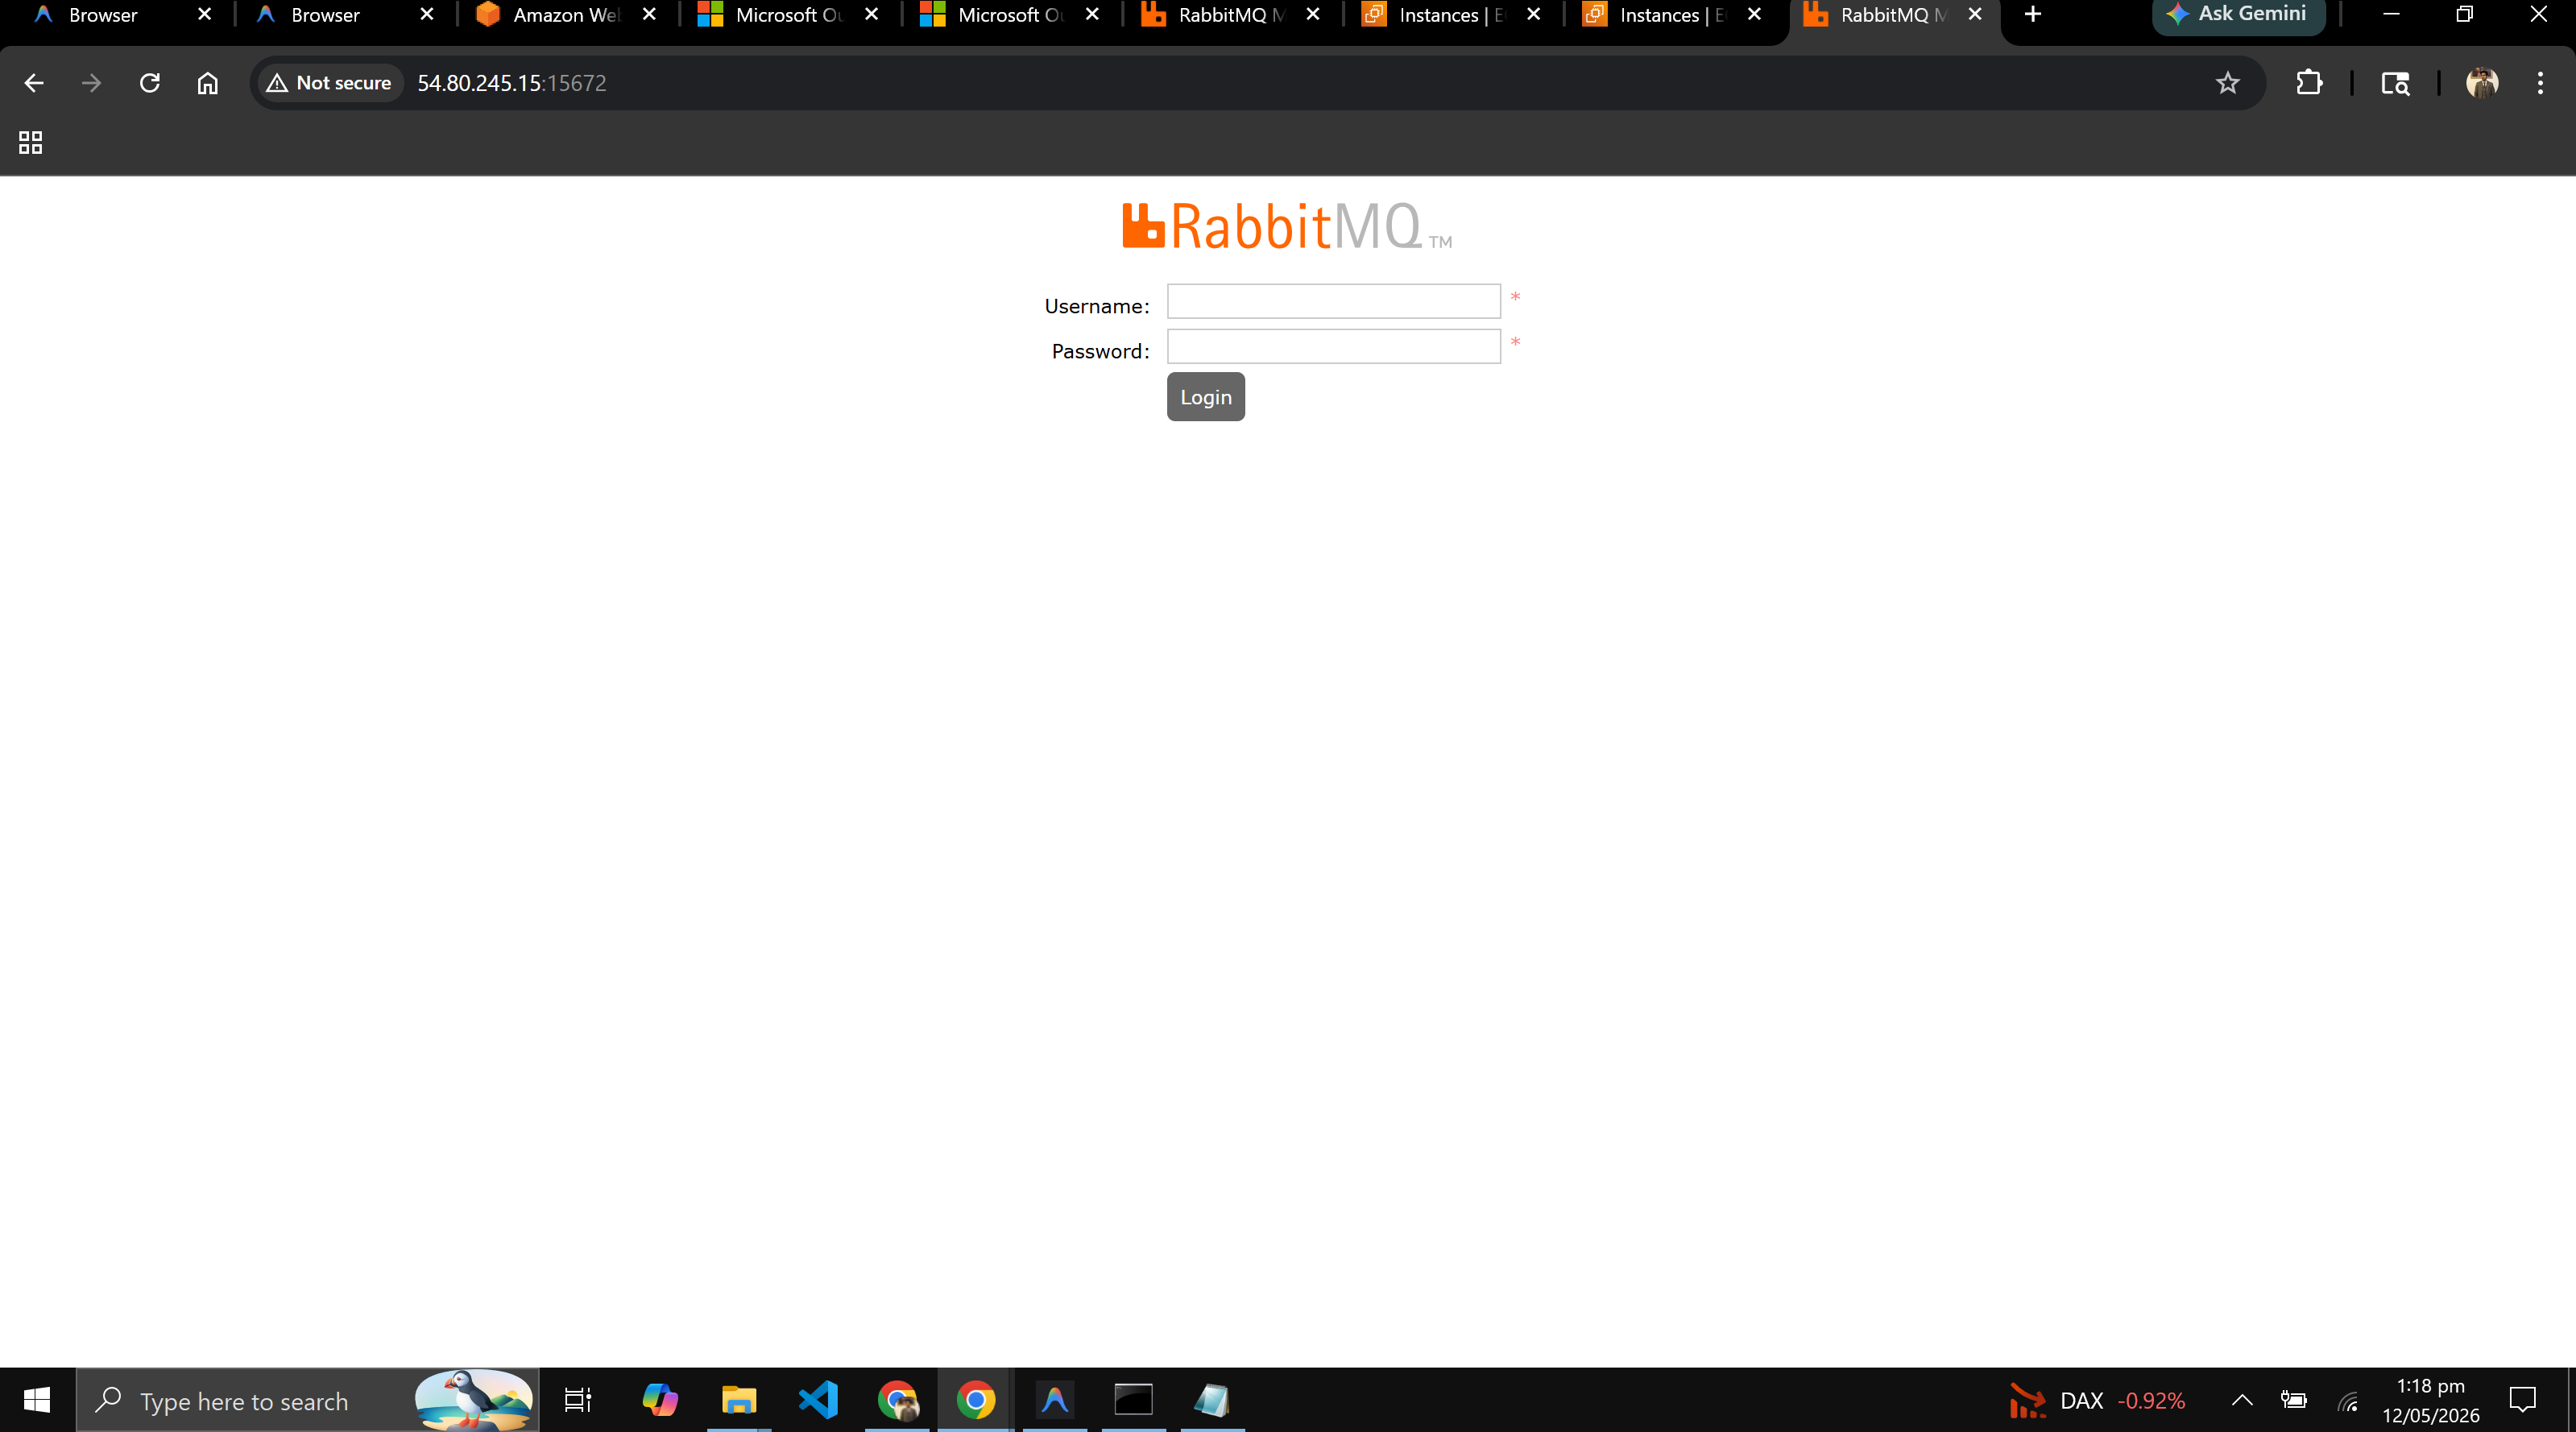
\includegraphics[width=0.95\linewidth]{exam_screenshots/login_on_ec2.png}
  \caption{Remote Verification: Successful Cloud JWT-Session Creation via EC2 IP}
  \label{fig:ec2_login_verification}
\end{figure}

As proven in Figure~\ref{fig:ec2_login_verification}, the client successfully authenticates against the live AWS instance and retrieves their signed JWT token securely.

\newpage

% ==========================================
% SECTION 6: CONCLUSION & TAKEAWAYS
% ==========================================
\section{Project Conclusion \& Cloud Engineering Takeaways}
All required lab parameters and learning outcomes for the CE408L Final Exam have been successfully met:

\begin{enumerate}
  \item \textbf{Decoupled Event-Driven Microservices}: Used RabbitMQ to decouple real-time database transactions (Event Service) from file-append operations (Notification Service).
  \item \textbf{Docker Orchestration}: Automated multi-container configuration through customized Alpine-based Dockerfiles and networks, ensuring portability.
  \item \textbf{AWS Production Deployment}: Gained hands-on proficiency in provisioning core cloud building blocks, including Virtual Private Clouds (VPC), security group rules, public Elastic IP mappings, and EBS attachments.
  \item \textbf{Lakehouse Log Ingestion}: Appended structured JSON logging metadata asynchronously to simulate massive enterprise data collection pipelines.
\end{enumerate}

The finalized microservices stack is fully active, tested, and ready for review on the public AWS EC2 instance.

\begin{table}[H]
  \centering
  \caption{Consolidated Microservices Architecture and Cloud Specifications}
  \begin{tabularx}{\linewidth}{l X l l}
    \toprule
    \textbf{Service Name} & \textbf{Docker Suffix / Container Name} & \textbf{Internal Port} & \textbf{Public Port (EC2)} \\
    \midrule
    \textbf{Postgres DB} & \texttt{postgres\_294} & \texttt{5432} & \textit{Shielded} \\
    \textbf{RabbitMQ Broker} & \texttt{rabbitmq\_294} & \texttt{5672} / \texttt{15672} & \texttt{15672} (Admin Dashboard) \\
    \textbf{Auth Microservice} & \texttt{auth\_service\_294} & \texttt{5001} & \texttt{5001} (Register/Login) \\
    \textbf{Event Microservice} & \texttt{event\_service\_294} & \texttt{5002} & \texttt{5002} (Secure Events) \\
    \textbf{Notification Daemon} & \texttt{notification\_service\_294} & \textit{Daemon} & \textit{Background Consumer} \\
    \bottomrule
  \end{tabularx}
  \label{tab:specs}
\end{table}

\end{document}
